\documentclass[../Document.tex]{subfiles}
\graphicspath{{\subfix{../images/}}}

\begin{document}


\section{Context-Free Grammar}
\label{sec:intro/cfg}
A \acrlong{cfg} is a set of rewrite rules used to generate strings.
Formally, grammar $\mathcal{G} = (\mathcal{N}, \Sigma, \mathcal{R}, S)$ is defined, respectively, by a set of nonterminal symbols $\mathcal{N}$, a set of terminal symbols (its alphabet) $\Sigma$, a set of production rules $\mathcal{R}$, and a start symbol $S$.
We denote $L(\mathcal{G})$ the language recognized by $\mathcal{G}$ \ie the set of strings that grammar can generate. 
According to Chomsky's classification, there are many types of grammars, ranging from least to most restrictive: Recursively Enumerable (Type-0), Context-Sensitive (Type-1), Context-Free (Type-2) and Regular (Type-3).
For a grammar to qualify as context-free, its production rules must respect two restrictions: the left-hand side of the production must be a single nonterminal, and the right-hand side must be a string of terminals and nonterminals.

The classic example of a \gls{cfg} is one where we match opening and closing parentheses. This becomes necessary later to ensure the validity of the generated molecules.

As an example of a \gls{cfg}, take the grammar defined as follows:

\begin{align*}
    \mathcal{N} &= \{S,A,B,C\}\\
    \Sigma &= \{\langle,\rangle\}\\
    \mathcal{R} &= \{\ \circled{1}\ S \rightarrow SS ,\ \circled{2}\ S \rightarrow AC ,\ \circled{3}\ S \rightarrow BC ,\ \circled{4}\ B \rightarrow AS ,\ \circled{5}\ A \rightarrow \langle ,\ \circled{6}\ C \rightarrow \rangle \}\\
    S &= S\\
\end{align*}

This context-free grammar recognizes correctly bracketed words such as ``$\langle \langle \rangle \rangle$'', obtained by the successive application of rules: 
$S \stackrel{3}{\rightarrow} BC \stackrel{4}{\rightarrow} ASC \stackrel{6}{\rightarrow} AS\rangle \stackrel{2}{\rightarrow} AAC\rangle \stackrel{5}{\rightarrow} A\langle C\rangle \stackrel{6}{\rightarrow} A \langle \rangle \rangle \stackrel{5}{\rightarrow} \langle \langle \rangle \rangle$.
Some of these rules could have been applied in a different order, but all such orderings correspond here to the same parse tree (the red one in Figure~\ref{fig:parseTrees}).

\begin{figure}[ht]
    \centering
    \scalebox{0.75}{
    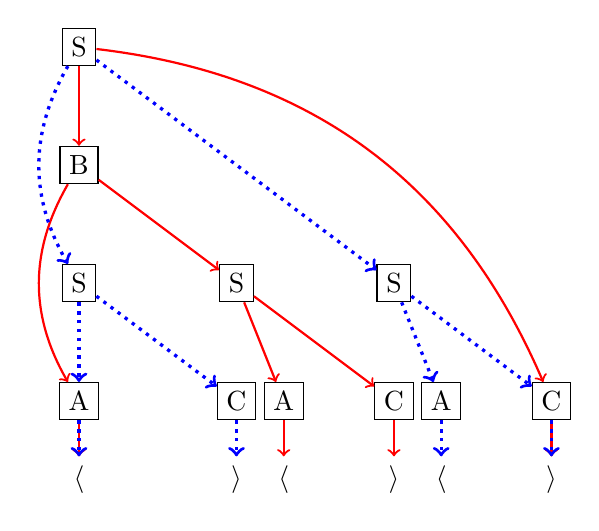
\begin{tikzpicture}
        \begin{scope}[every node/.style={draw}]
            \node (S4) at (1,5.5) {S};
            \node (B) at (1,4) {B};
            \node (S21) at (1,2.5) {S};
            \node (S22) at (3,2.5) {S};
            \node (S23) at (5,2.5) {S};
            \node (A1) at (1,1) {A};
            \node (A2) at (3.6,1) {A};
            \node (A3) at (5.6,1) {A};
            \node (C2) at (3,1) {C};
            \node (C3) at (5,1) {C};
            \node (C4) at (7,1) {C};
        \end{scope}
        \begin{scope}[every node/.style={}]
            \node (a1) at (1,0) {$\langle$};
            \node (a2) at (3.6,0) {$\langle$};
            \node (a3) at (5.6,0) {$\langle$};
            \node (c2) at (3,0) {$\rangle$};
            \node (c3) at (5,0) {$\rangle$};
            \node (c4) at (7,0) {$\rangle$};
        \end{scope}
        \begin{scope}[every edge/.style={draw=red, thick}]
        %              every node/.style={fill=white,circle}, 
        %    \path [->] (S4) edge node {$5$} (B);
            \path [->] (S4) edge  (B);
            \path [->] (S4) edge[bend left=30]  (C4); 
            \path [->] (B) edge[bend right=30] (A1);   
            \path [->] (B) edge (S22);
            \path [->] (S22) edge (A2);
            \path [->] (S22) edge (C3);
            \path [->] (A1) edge (a1);
            \path [->] (A2) edge (a2);
            \path [->] (C3) edge (c3);
            \path [->] (C4) edge (c4);
        \end{scope}
        \begin{scope}[every edge/.style={draw=blue,very thick,dotted}]
            \path [->] (S4) edge[bend right=30] (S21); 
            \path [->] (S4) edge (S23);
            \path [->] (S21) edge (A1);
            \path [->] (S21) edge (C2);
            \path [->] (S23) edge (A3);
            \path [->] (S23) edge (C4);
            \path [->] (A1) edge (a1);
            \path [->] (C2) edge (c2);
            \path [->] (A3) edge (a3);
            \path [->] (C4) edge (c4);
        \end{scope}
    \end{tikzpicture}
    }
    \caption[Grammar parse tree]{Grammar parse tree for the two words of length 4 recognized by the grammar shown in Section~\ref{sec:intro/cfg}. The first word is in red, the second is in blue.}
    \label{fig:parseTrees}
\end{figure}



\subsection{Chomsky Normal Form}
\askGilles{Should I move this to when I talk about grammars and explain how the algo works there instead?}
A grammar is said to be in Chomsky Normal Form if it follows a few additional rules on top of those of a \gls{cfg}. No production may contain the null symbol $\epsilon$ and the right-hand side of any production must be either: a single terminal or two nonterminals. The following \gls{cfg} could be converted to be in Chomsky Normal Form by applying four steps.

\begin{align*}
    \mathcal{N} &= \{S,X,Y,Z\}\\
    \Sigma &= \{a,b\}\\
    \mathcal{R} &= \{ S \rightarrow XYZ ,\  X \rightarrow aXb ,\  X \rightarrow \epsilon ,\  Y \rightarrow aa ,\   Y \rightarrow bb ,\ Y \rightarrow X ,\ Z \rightarrow abba ,\ Z \rightarrow XabY \}\\
    S &= S\\
\end{align*}

\begin{enumerate}
    \setcounter{enumi}{-1}
    \item Initial grammar
        \begin{align*}
            S &\rightarrow XYZ\\
            X &\rightarrow aXb \mid \epsilon\\
            Y &\rightarrow X \mid aa \mid bb\\
            Z &\rightarrow XabY \mid abba\\
        \end{align*}
    \item Remove null productions
        \begin{align*}
            S &\rightarrow XYZ \mid XZ \mid YZ \mid Z\\
            X &\rightarrow aXb \mid ab\\
            Y &\rightarrow X \mid aa \mid bb\\
            Z &\rightarrow XabY \mid Xab \mid abY \mid ab \mid abba\\
        \end{align*}
    \item Replace unit productions
        \begin{align*}
            S &\rightarrow XYZ \mid XZ \mid YZ \mid XabY \mid Xab \mid abY \mid ab \mid abba\\
            X &\rightarrow aXb \mid ab\\
            Y &\rightarrow aXb \mid ab \mid aa \mid bb\\
            Z &\rightarrow XabY \mid Xab \mid abY \mid ab \mid abba\\
        \end{align*}
    \item Shorten the right-side to two tokens
        \begin{align*}
            S &\rightarrow XC \mid XZ \mid YZ \mid XD \mid XE \mid EY \mid ab \mid EF\\
            X &\rightarrow aG \mid ab\\
            Y &\rightarrow aG \mid ab \mid aa \mid bb\\
            Z &\rightarrow XD \mid XE \mid EY \mid ab \mid EF\\
            C &\rightarrow YZ\\
            D &\rightarrow EY\\
            E &\rightarrow ab\\
            F &\rightarrow ba\\
            G &\rightarrow Xb\\
        \end{align*}
    \item Create unit productions for terminal tokens
        \begin{align*}
            S &\rightarrow XC \mid XZ \mid YZ \mid XD \mid XE \mid EY \mid AB \mid EF\\
            X &\rightarrow AG \mid AB\\
            Y &\rightarrow AG \mid AB \mid AA \mid BB\\
            Z &\rightarrow XD \mid XE \mid EY \mid AB \mid EF\\
            A &\rightarrow a\\
            B &\rightarrow b\\
            C &\rightarrow YZ\\
            D &\rightarrow EY\\
            E &\rightarrow AB\\
            F &\rightarrow BA\\
            G &\rightarrow XB\\
        \end{align*}
\end{enumerate}


\end{document}